\documentclass[12pt,a4paper,twoside]{article}
\usepackage[utf8]{inputenc}
\usepackage[english]{babel}
\usepackage[e]{esvect}
\usepackage{verbatim}
%\usepackage[landscape]{geometry}
\usepackage{tikz}
\usetikzlibrary{mindmap}
\usepackage{metalogo}
\usepackage{amsmath}
\usepackage{amsfonts}
\usepackage{amssymb}
\usepackage{makeidx}
\usepackage{graphicx}
\usepackage{lmodern}
\usepackage[left=2cm,right=1.5cm,top=2cm,bottom=2cm]{geometry}
\usepackage{pdfpages}
\usepackage[left]{lineno}
\usepackage{url}
%\usepackage{fullpage}

\usepackage[colorlinks=true,linkcolor=blue,anchorcolor=black,citecolor=black,filecolor=black,menucolor=black,runcolor=black,urlcolor=black]{hyperref}
\usepackage{hyperref}
\usepackage{tikz}
\usepackage{setspace}
\usepackage{caption}


\usetikzlibrary{shapes.geometric,arrows}
\tikzstyle{startstop} = [rectangle, rounded corners, minimum width=3cm, minimum height=1cm, text centered, draw=black, fill=red!30]
\tikzstyle{io}        = [trapezium, trapezium left angle=70, trapezium right angle=110, minimum width=1cm, minimum height=1cm, text centered, draw=black, fill=blue!30]
\tikzstyle{process}   = [rectangle, minimum width=3cm, minimum height=1cm, text centered, draw=black, fill=orange!30]
\tikzstyle{decision}  = [diamond, minimum width=3cm, minimum height=1cm, text centered, draw=black, fill=green!30]
\tikzstyle{arrow}     = [thick,->,>=stealth]
\usetikzlibrary{shapes,arrows,matrix,      % For easy node positioning
	fit,         % For easily fitting nodes inside another one
	positioning}
\usepackage[utf8]{inputenc}
\usepackage[english]{babel}
\setlength{\parindent}{0em}
\setlength{\parskip}{1em}
\renewcommand{\baselinestretch}{1.0}
\renewcommand{\familydefault}{\sfdefault}
%\pagenumbering{gobble}

%%%%%%%%%%%%%%%%%%%%%% Programming CodePackages %%%%%%%%%%%%%%%%%%%%%%%%%%%%%%%%%%%
%%%%%%%%%%%%%%%%%%%%%%%%%%%%%%%%%%%%%%%%%%%%%%%%%%%%%%%%%%%%%%%%%%%%%%%%%%%%%%%%%%%

\usepackage{xcolor}
\usepackage{listings}
\definecolor{mGreen}{rgb}{0,0.6,0}
\definecolor{mGray}{rgb}{0.5,0.5,0.5}
\definecolor{mPurple}{rgb}{0.58,0,0.82}
\definecolor{backgroundColour}{rgb}{0.95,0.95,0.92}

\lstdefinestyle{CStyle}
{
	backgroundcolor=\color{backgroundColour},   
	commentstyle=\color{mGreen},
	keywordstyle=\color{magenta},
	numberstyle=\tiny\color{mGray},
	stringstyle=\color{mPurple},
	basicstyle=\footnotesize,
	breakatwhitespace=false,         
	breaklines=true,                 
	captionpos=b,                    
	keepspaces=true,                 
	numbers=left,                    
	numbersep=5pt,                  
	showspaces=false,                
	showstringspaces=false,
	showtabs=false,                  
	tabsize=2,
	language=C
}



\begin{document}
\begin{titlepage}

\newcommand{\HRule}{\rule{\linewidth}{0.5mm}} % Defines a new command for the horizontal lines, change thickness here

\center % Center everything on the page
 
%----------------------------------------------------------------------------------------
%	HEADING SECTIONS
%----------------------------------------------------------------------------------------

\textsc{\LARGE IIT HYDERABAD}\\[1.5cm] % Name of your university/college
\textsc{\Large INTRODUCTION TO AI AND ML}\\[0.5cm] % Major heading such as course name
%\textsc{\large ASSIGNMENT}\\[0.5cm] % Minor heading such as course title

%----------------------------------------------------------------------------------------
%	TITLE SECTION
%----------------------------------------------------------------------------------------

\HRule \\[0.4cm]
{ \huge \bfseries ASSIGNMENT}\\[0.4cm] % Title of your document
\HRule \\[1.5cm]
 
%----------------------------------------------------------------------------------------
%	AUTHOR SECTION
%----------------------------------------------------------------------------------------

\begin{minipage}{0.4\textwidth}
\begin{flushleft} \normalsize
\emph{Author:}\\
NAMRATA MISHRA\\
ee21mtech14023% Your name
\end{flushleft}
\end{minipage}
~
\begin{minipage}{0.4\textwidth}
\begin{flushright} \normalsize
\emph{Supervisor:} \\
Prof SHIV GOVIND SINGH % Supervisor's Name
\end{flushright}
\end{minipage}\\[2cm]

% If you don't want a supervisor, uncomment the two lines below and remove the section above
%\Large \emph{Author:}\\
%John \textsc{Smith}\\[3cm] % Your name

%----------------------------------------------------------------------------------------
%	DATE SECTION
%----------------------------------------------------------------------------------------

{\large \today}\\[2cm] % Date, change the \today to a set date if you want to be precise

%----------------------------------------------------------------------------------------
%	LOGO SECTION
%----------------------------------------------------------------------------------------


\includegraphics[scale=0.8]{logo iit h.png}\\ % Include a department/university logo - this will require the graphicx package
 
%----------------------------------------------------------------------------------------

\vfill % Fill the rest of the page with whitespace

\end{titlepage}



\section{PROBLEM}
The line joining the points (-6,8) and (8,-6) is divided into four equal parts; Find the coordinates of the points of section.
\section{SOLUTION}
We will be using matrix approach for calculating the coordinates of the points of section which is divided into four equal parts.\\
$\begin{bmatrix}
\vec{x1}\\
\vec{y1}
\end{bmatrix}$
= $\frac{1}{4}$
$\begin{bmatrix}
-6 & 8\\
8 & -6
\end{bmatrix}$
$\begin{bmatrix}
3\\
1
\end{bmatrix}$
= $\begin{bmatrix}
-10/4\\
18/4
\end{bmatrix}$
=
$\begin{bmatrix}
-5/2\\
9/2
\end{bmatrix}$


Points x1,y1 divides line in ratio 3:1\\

$\begin{bmatrix}
\vec{x2}\\
\vec{y2}
\end{bmatrix}$
= $\frac{1}{2}$ 
$\begin{bmatrix}
-6 & 8\\
8 & -6
\end{bmatrix}$
$\begin{bmatrix}
1\\
1
\end{bmatrix}$
=
$\begin{bmatrix}
2/2\\
2/2
\end{bmatrix}$
=
$\begin{bmatrix}
1\\
1
\end{bmatrix}$

Points x2,y2 divides lines in ratio 1:1\\

$\begin{bmatrix}
\vec{x3}\\
\vec{y3}
\end{bmatrix}$
= $\frac{1}{4}$
$\begin{bmatrix}
-6 & 8\\
8 & -6
\end{bmatrix}$
$\begin{bmatrix}
1\\
3
\end{bmatrix}$
= $\begin{bmatrix}
18/4\\
-10/4
\end{bmatrix}$
= $\begin{bmatrix}
9/2\\
-5/2
\end{bmatrix}$

Points x3,y3 divides lines in ratio 1:3\\
\section{PLOT OBTAINED FROM PYTHON CODE}
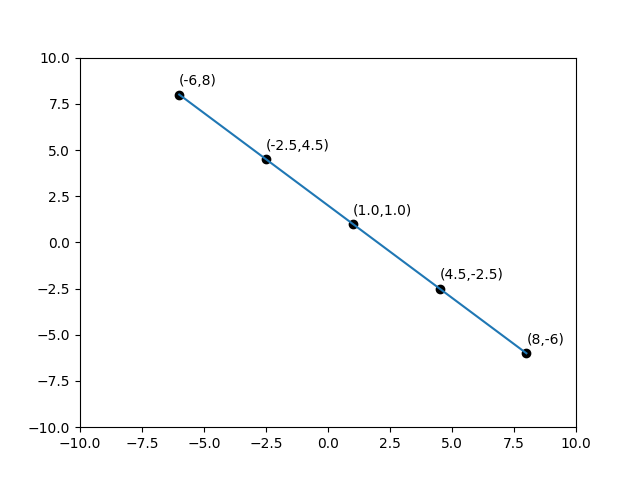
\includegraphics[scale=0.5]{Figure_1.png}
\section{CONCLUSION}

The points $(\vec{x1} \vec{y1}), (\vec{x2} \vec{y2}), (\vec{x3} \vec{y3})$divides the lines into four parts in ratio (3:1) (1:1) (1:3).
The points  $(\vec{x1}  \vec{y1})=(-2.5,4.5), ( \vec{x2} \vec{y2})=(1,1), ( \vec{x3} \vec{y3})=(4.5,-2.5)$

https://www.overleaf.com/project/6128ee907ed3661ebeed4bc8
\end{document}
 








